% \documentclass[a4paper,10pt]{article}

% \usepackage[utf8]{inputenc}
% \usepackage{natbib}
% %\usepackage[vmargin=2cm]{geometry}
% \usepackage{fullpage}

% \setlength{\bibsep}{1pt}
% \usepackage{graphicx}
% \graphicspath{{Figures/}}

% \usepackage{hyperref}
% \hypersetup{
%   colorlinks, linkcolor=red
% }

% \renewcommand{\bibfont}{\small}


% %\title{Project report - Object Recognition and Computer vision}
% \title{%
% 	\huge{Training Restricted Boltzmann Machines}\\ \bigbreak
%   	\Large{Project report}\\ 
%   	\Large{Probabilistic Graphical Models - MVA}
% }
% \author{Chaimaa Kadaoui, Othman Sbai, Xi Shen}
% \date\today

\documentclass{article}
\PassOptionsToPackage{numbers, compress}{natbib}

% if you need to pass options to natbib, use, e.g.:
% \PassOptionsToPackage{numbers, compress}{natbib}
% before loading nips_2016
%
% to avoid loading the natbib package, add option nonatbib:
% \usepackage[nonatbib]{nips_2016}

\usepackage[final]{nips_2016}

% to compile a camera-ready version, add the [final] option, e.g.:
% \usepackage[final]{nips_2016}

\usepackage[utf8]{inputenc} % allow utf-8 input
\usepackage[T1]{fontenc}    % use 8-bit T1 fonts
\usepackage[colorlinks=false]{hyperref}       % hyperlinks
% \hypersetup{
%     colorlinks = false,
%     linkbordercolor = {white},
% }
\usepackage{url}            % simple URL typesetting
\usepackage{booktabs}       % professional-quality tables
\usepackage{amsfonts}       % blackboard math symbols
\usepackage{nicefrac}       % compact symbols for 1/2, etc.
\usepackage{microtype}      % microtypography
\usepackage[]{amsmath}
\usepackage[]{graphicx}
\usepackage[]{float}
\graphicspath{{Figures/}}
\usepackage{algorithm}
\usepackage{algorithmic}
\usepackage{caption}
\usepackage{subcaption}
\usepackage{fullpage}


\DeclareMathOperator*{\argmax}{\arg\!\max}
\title{Restricted Boltzmann Machines}

% The \author macro works with any number of authors. There are two
% commands used to separate the names and addresses of multiple
% authors: \And and \AND.
%
% Using \And between authors leaves it to LaTeX to determine where to
% break the lines. Using \AND forces a line break at that point. So,
% if LaTeX puts 3 of 4 authors names on the first line, and the last
% on the second line, try using \AND instead of \And before the third
% author name.

\author{
  Chaimaa Kadaoui  \\
  \texttt{chaimaa.kadaoui\thanks{mail extension @eleves.enpc.fr for all authors}} \\
  \And
  Othman SBAI \\
  \texttt{othman.sbai} \\
  \And
   Xi Shen\\
  \texttt{xi.shenxi} \\
}


\begin{document}

\maketitle
\section{Abstract}
For our project in Probabilistic Graphical Models course, we studied the use and the training of Restricted Boltzmann Machines as an instance of undirected graphical models. We mainly base our approach on the practical guide for training Restricted Boltzmann Machines (Hinton 2010~\cite{hinton2010practical}). We start by an introduction to RBM and the interest that they have raised in the last years, then we define the theoretical aspects of main training methods of RBM. Finally we present our results by comparing our implementation of training RBM to an implementation from another deep learning library, on two popular image datasets MNIST and CIFAR-10. We show our convergence results and investigate the influence of different parameters of the training algorithm.


%-----------------------------------------------
%	Intro
%-----------------------------------------------

\section{Introduction}
\subsection{Definition of an RBM}

A Restricted Boltzmann Machine (RBM) is an undirected energy-based probabilistic graphical model which can be seen as a two layer neural network (visible and hidden units). RBMs can be used to model and learn important aspects of a probability distribution of a training data. They are called restricted, because we impose restrictions on the network topology, by allowing only connections between units of different layers. RBM are energy-based, since they define probability distribution through an energy function. Learning corresponds to shaping the energy so that desirable configurations have a low energy and thus maximize probability of training data under the model. Maximum likelihood learning is challenging for undirected graphical models because MLE parameters cannot be found analytically and the log likelihood gradient based optimization is not tractable. This optimization requires obtaining samples through Markov Chain Monte Carlo, which is computationally demanding.

% what about EM algorithm ?

\subsection{Interest in RBM}

A major interest have been dedicated to directed graphical models with one layer of observed variables and one or more layers of hidden variables such Mixture of Gaussians, probabilistic PCA, factor analysis, latent dirichlet analysis LDA... However, the undirected two layered analogue which was first introduced and called Harmonium by \cite{smolensky1986information} and renamed as "Restricted Boltzmann Machines" by \cite{hinton2002training} have also seen advances through new training methods, which unlike directed graphical models, makes inference and learning very fast. 

%https://papers.nips.cc/paper/2672-exponential-family-harmoniums-with-an-application-to-information-retrieval.pdf
%http://www.cs.toronto.edu/~hinton/absps/tr00-004.pdf

\section{Applications of RBM}
% to be reformulated /.. copied ../
Restricted Boltzmann machines have successfully been applied to problems involving high dimensional data such as images, text  \cite{hinton2006fast}, \cite{vincent2010stacked} as unsupervised feature extractors.

Recent developments have demonstrated the capacity of RBM to be powerful generative models, able to extract useful features from input data or construct deep artificial neural networks. In this setting they can be seen as good preprocessing or initialization for some other models. They can also be used as self-contained classifiers as shown in \cite{larochelle2012learning}.

\begin{itemize}
		\item \textbf{RBM as a generative model}: learns and generates samples from data distribution 
		\item \textbf{RBM as feature extractor}: unsupervised feature extraction from data, instead of handcrafting features 
		\item \textbf{RBM for computer vision}: such as object recognition, image denoising and inpainting.
		\item \textbf{RBM for collaborative filtering}: given a set of N users and M movies, recommend movies to the users.
	\end{itemize}

%-----------------------------------------------
%	Theory of RBM
%-----------------------------------------------

\section{Theory of RBM}

\subsection{Definition of RBM}
Restricted Boltzmann Machines are particular instance of undirected graphical models inspired by neural networks, where the units are organized in two layers.

\begin{itemize}
    \item The visible layer $ \mathbf{x} $ which contains all the visible nodes.
    \item The hidden layer $ \mathbf{h} $ with all the latent variables.
\end{itemize}

It is \emph{restricted} because no connections between nodes of the same layer are allowed. Each node of one layer is connected to all the other nodes of the other layer ($h_j \leftrightarrow x_k$). The matrix $W$ characterizes the connections between the two layers: $ W_{j,k} $ is the value for the connection between $h_j$ and $x_k$. For simplification, we suppose that the variables $ \mathbf{x} $ and $ \mathbf{h} $ are binary.

\begin{figure}
\centering

\includegraphics[width=0.5\textwidth]{rbm.png}
\label{fig:RBM}
\caption{The network graph of an RBM}
\end{figure}

\subsection{Energy and probability}
\label{subsec:energy}
We introduce the two bias vectors $c$ and $b$ to define the energy of this graph:

\[ E(x,h) = -h^\top W x - c^\top x - b^\top h \]

We can write the joint probability of $ \mathbf{x} $ and $ \mathbf{h} $ as: 

\[ p(x,h) = \frac{1}{Z} \exp(-E(x,h)) \]

$Z$ is the partition parameter which can be computed by calculating all the possibles values of $ \mathbf{x} $  and $ \mathbf{h} $. In practice, this parameter is intractable.

We see that to increase the probability, we want to decrease the energy. We have:
 
\begin{itemize}
    \item if $c_k < 0$ and $x_k = 1$, the energy is higher; therefore we prefer having $x_k = 0$ (the probability of $x_k = 1$ decreases).
    \item if $c_k > 0$, similarly, we prefer $x_k = 1$ over $x_k = 0$.
\end{itemize}

We apply the same arguments for $b$ and $W$ and deduce similar interpretations of theses parameters.

%-----------------------------------------------
%	Inference
%-----------------------------------------------

\section{Inference: Conditional inference}

Because $p(x)$ is intractable, the only possible type of inference is computing conditional inference. We will prove that computing the conditional probabilities $p(x|h)$ and $p(h|x)$ is easy.

Because of the construction of the graph, the variables $h_1, \hdots, h_H$ are independant conditionally on $\mathbf{x}$: \[p(h|x) = \prod_j p(h_j|x)\]

We can also prove that given $\mathbf{x}$, $h_j$ follows a Bernoulli:

\[ p(h_j=1|x) = sigm(b_j + W_{j.}x)\]

$ W_{j.}$ is the j-th row of $W$ and $sigm$ defines the sigmoid function: $$sigm(x) = \frac{1}{1+e^{-x}}$$

We can prove that either by derivation of  $p(h|x)$ or by applying the \emph{Local Markov Property}: $p(z_i|z_j, \; j \neq i) =  p(z_i|\mathcal{N}(z_i))$.

\subsection{Free energy}

To have a better understanding of the parametrs $W \;, c \;, b$, let's introduce the concept of free energy. Using a marginalization and some derivations, we can write the probability $p(x)$ as :

\[ p(x) = \sum_h p(x,h) = \exp\left(c^\top x + \sum_{j=1}^H \log\left( 1+\exp(b_j + W_{j.}x) \right) \right) / Z \]

The function $u \mapsto \log\left( 1+\exp(u) \right)$ is called \texttt{softplus} and is a soft approximation of $u \mapsto \max(u,0)$. \\

We can see that $p(x) = \exp\left(-F(x)\right) / Z$ where $F$ is the free energy. We want to increase the probability of our data $x$ and thus decreases its energy. Let's look at each term of this energy:

\begin{itemize}
    \item As seen in the previous subsection (\ref{subsec:energy}), the sign of $c_k$ impacts wether $x_k$ would be a 0 or 1. Thus, having $c^\top x$ in the probability means that we want $\mathbf{x}$ and the bias $c$ to be aligned. This bias characterizes the probability.
    \item Similarly, $\mathbf{x}$ and $W_{j.}$ should align for each $j$. And we can see $b_j$ as a control parameter: $W_{j.}x$ has to be big enough to have $b_j + W_{j.}x > 0 $.  Therefors, we can considers the hidden variables as features and $b_j$ the bias for each feature (it defines the importance of each feature). The goal of the RBM is to represent meaningful features.
\end{itemize}

%-----------------------------------------------
%	Contrastive Divergence
%-----------------------------------------------

\section{Contrastive divergence method for training RBM efficiently}

To train the RBM with our data $\mathbf{x}^{(t)}$, we would like to minimize the average loss:

\[ \frac{1}{T} \sum_t l(f(\mathbf{x}^{(t)})) =  \frac{1}{T} \sum_t - \log p(\mathbf{x}^{(t)}) \]

We want to apply a stochastic gradient descent. We derive each term of the sum with respect to our model parameter $\theta$ as follow (where $\mathbb{E}_h$ and $\mathbb{E}_{x,h}$ are expectations of $h$ and $(x,h)$ respectively):

\[ \frac{\partial - \log p(\mathbf{x}^{(t)})}{\partial \theta} = \mathbb{E}_h \left[ \frac{\partial E(\mathbf{x}^{(t)} ,h)}{\partial \theta} | \mathbf{x}^{(t)} \right] - \mathbb{E}_{x,h} \left[ \frac{\partial E(\mathbf{x} ,h)}{\partial \theta} \right] \]

The first term is called the \emph{positive phase} and the second term the {negative phase}. Because of the difficulty to compute the seconde term, we will use an algorithm called \emph{Contrastive Divergence}. The idea is:

\begin{enumerate}
    \item We estimate the expectation $\mathbb{E}_{x,h}$ by sampling a single point $\mathbf{\tilde x}$.
    \item To do so, we use Gibbs sampling in chain (we apply it $k$ times).
    \item We initialize our Gibbs sampling with $\mathbf{x^{(t)}}$.
\end{enumerate}

Therefore we can rewrite each term as:

\[ \mathbb{E}_h \left[ \frac{\partial E(\mathbf{x}^{(t)} ,h)}{\partial \theta} | \mathbf{x}^{(t)} \right] \simeq \frac{\partial E(\mathbf{x}^{(t)} ,h(\mathbf{x}^{(t)}))}{\partial \theta} \]

\[ \mathbb{E}_{x,h} \left[ \frac{\partial E(\mathbf{x} ,h)}{\partial \theta} \right] \simeq \frac{\partial E(\mathbf{\tilde x} ,h(\mathbf{\tilde x}))}{\partial \theta} \]

The goal is to minimize the energy of our training data and to increase the energy of our samplings at each iteration until we have samplings similar to our training data.

We define for a given $x$, the vector $h(x)$ as:

\[ h(x) =
\begin{bmatrix}
    p(h_1 = 1 | x)  \\
    \vdots \\
    p(h_H = 1 | x)
\end{bmatrix}
\]

$$ h(x) = sigm(b + Wx) $$

Let's look at the derivative of the energy $E$ with respect to $W$, we can prove that:

\[ \nabla_{\mathbf{W}} E(x,h) = -h(x) x^\top \]

Therefore, we can update $W$ ($\alpha$ is the step of the gradient descent):

\[ W = W + \alpha \left( h(\mathbf{x^{(t)}})\mathbf{x^{(t)}}^\top - h(\mathbf{\tilde x})\mathbf{\tilde x}^\top \right) \]

We do the same to update $b$ and $c$:

\[ b = b + \alpha \left(h(\mathbf{x^{(t)}}) - h(\mathbf{\tilde x}) \right)  ~~~~~~~~~,~~~~~~~~~ c = c + \alpha \left(\mathbf{x^{(t)}} - \mathbf{\tilde x} \right)\]

%\[  \]

\begin{enumerate}
    \item For each $\mathbf{x^{(t)}}$
    \begin{enumerate}
        \item Generate sample $ \tilde{\mathbf{x}} $ using $ k $ steps Gibbs sampling starting at $\mathbf{x^{(t)}}$
        \item Update parameters:
        \begin{itemize}
            \item $ W = W + \alpha \left( h(\mathbf{x^{(t)}})\mathbf{x^{(t)}}^\top - h(\mathbf{\tilde x})\mathbf{\tilde x}^\top \right) $
            \item $ b = b + \alpha \left(h(\mathbf{x^{(t)}}) - h(\mathbf{\tilde x}) \right) $
            \item $ c = c + \alpha \left(\mathbf{x^{(t)}} - \mathbf{\tilde x} \right) $
        \end{itemize}
    \end{enumerate}
    \item Go back to step 1 until stopping criterion
\end{enumerate}

The more steps we use for Gibbs sampling, the lower is the bias of our estimate. However it takes more time to compute. In practice, taking $k=1$ works well to initialize the parameters of the algorithm.

% \subsection*{Persistent Contrastive Divergence}

% The main issue of k-steps Gibbs sampling is that starting from a point $\mathbf{x^{(t)}}$, it won't wander far away from this point so we may miss a point with lower energy. Therefore we might be stuck in a local minimum unless we take a great $k$.

% To allow $\tilde{x}$ to wander further away from the training examples, at each iteration of the algorithm, we initialize the Gibbs sampling with the sample from the previous iteration.

\clearpage
\section{Implementation and results}

We implemented the RBM training algorithm in python (Github repository available at \footnote{https://github.com/sbaio/Restricted-Boltzmann-Machine}) and then we compared our implementation performance with an existing deep learning library using tensorflow (YADLT \cite{yadltGithub}), we applied it to the MNIST dataset (images of handwritten digits) and CIFAR-10 (color images of different classes). In the case of image data, each pixel is considered as a node; the intensity $p \in [0,1]$ of a pixel is considered as a probability. \\

\subsection{Implementation of RBM in python}

The implementation of RBM training consists of implementing the constrastive divergence learning strategy through Gibbs sampling. We only needed few steps of Contrastrive divergence for a good training. We compare the difference between using different values of k steps for CD-k algorithm \ref{subsubsec:CDk}.
We also used mini batches during training in order to compute the approximate gradient in every step. The influence of the batch size is studied in subsection \ref{subsubsec:BS}.

\subsection{Implementation of RBM in tensorflow using a GPU}

We use the implementation in tensorflow and python provided by Gabriele Angeletti as a library gathering many deep learning models and algorithms such as convolutional networks, RNN, RBM, Deep Belief Networks... We observe the difference in training time between the two implementations. The difference is not very important because of small batch size, and small matrices size in multiplication \cite{fatahalian2004understanding}: 25 seconds for training 1 epoch on GPU with batch size of 10 versus 35 to 40 seconds with our CPU implementation using numpy. 

\subsection{Convergence plot}

In general, it is difficult to directly evaluate the performances of RBM. This is due to the fact that the parameter $Z$ is intractable and we are unable to compute the average loss. A solution 

\subsection{Influence of different algorithm parameters}

\subsubsection{Influence of batch size}
\label{subsubsec:BS}

\subsubsection{Influence of number of hidden units}

As we can see in the figure \ref{fig:hidden}, the number of hidden units has a direct impact on the performance of the algorithm. By increasing the number of hidden units, we can decrease the average stochastic reconstruction. In the figure, we can see that clearly 100 hidden units isn't enough; however for bigger values the curves become closer. 

Since we deal with high dimensional data (images of abouts 1000 pixels each), we don't risk overfitting with a number of hidden units between 100 and 500 (the valiation loss is still below the training loss in each case). Hence, our main constraint for the choice of this parameter was the time complexity. We found that 200 or 300 was a good compromise between computing time and performances.

\begin{figure}
\centering
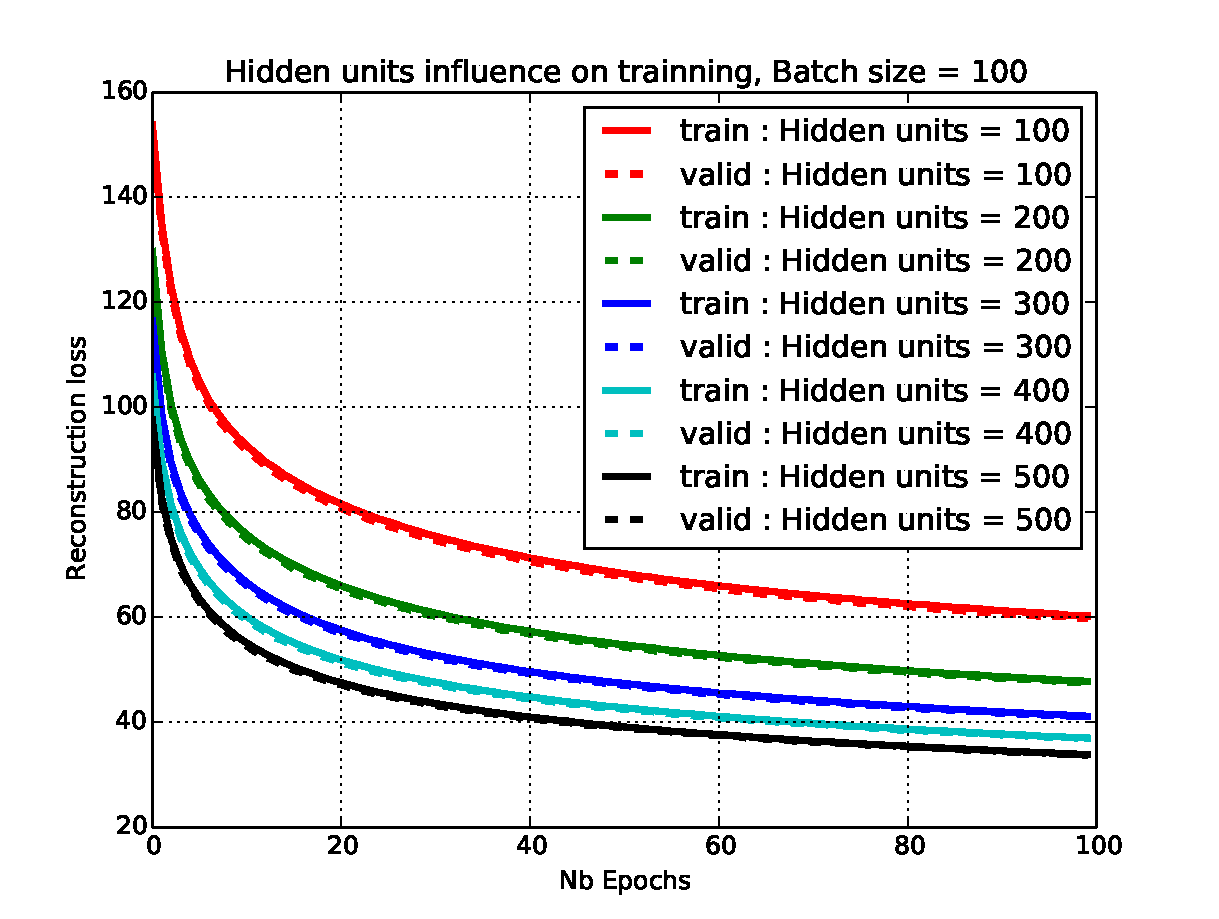
\includegraphics[width=0.75\textwidth]{hidden_units}
\label{fig:hidden}
\caption{Influence of the number of hidden units}
\end{figure}

% define the loss we are using
% compare the loss evolution over epochs while varying parameters 
% reconstruct hidden layers?
\subsubsection{Influence of number of steps in contrastive divergence algorithm}
\label{subsubsec:CDk}

\clearpage
\section{Conclusion and future work}



\clearpage
\nocite{*}
\bibliographystyle{plain}
\bibliography{biblio}


\end{document}



% overfitting ?
% convergence ?